\chapter{Methods}
\section{Participants}
In the present study, we had a total population of 42 subjects, equally divided into two groups: 21 individuals were part of the healthy control group, whilst the remaining 21 were patients who suffered from a cortical or subcortical stroke. The recruitment for the control group was made through several methods: in person, talking to alumni of the \href{https://www.experiencia.ub.edu/ca/}{Universitat de l'Experiència of Barcelona}, through personal contacts, and using the platform \href{https://www.sona-systems.com/}{Sonasystem}. 
On the other hand, to recruit participants who experienced a stroke we used a database previously employed in another study made in the \href{https://brainvitge.org/}{Cognition and Brain Plasticity Unit} for movement rehabilitation with music therapy. Furthermore, we were also able to present our study at \href{https://www.fundacioictus.com/}{Fundació Ictus}, where we could select more participants.  
The exclusion criteria in both groups were: no visual or auditory impairments and no pregnancy.

Participants of the two groups were matched by age and gender, where we can find a mean of 55,4 years old in the control group and of 56,4 for the stroke patients, with a non-significant difference (\textit{t} test: -0.299, \textit{p} value: .766). Likewise, the difference is gender did not result significantly different (\textit{t} test: 1.56, \textit{p} value: .127), even though higher participation of men compared to women can be observed in the stroke group and a preponderance of women compared to men can be observed in the control group. 
To both groups a questionnaire measuring the level of physical activity was administrated: an average of 7026,78 kilojoules a day was found for the control group, whilst for the stroke group it resulted of 5669,19 kJ/d, which results lower than the control group, but still without a significant difference (\textit{t} test: 1.06, \textit{p} value: .146). 
Regarding the stroke group, the clinical history of the patients was collected, founding the majority of patients with the injured left hemisphere, which affected their contralateral right extremity (\textit{N=}13 suffered the injury in the left hemisphere; \textit{N=}7 in the right hemisphere; \textit{N=}1 in both hemispheres; a database can be found in Table A.\ref{tab: Database stroke}). 
Participants signed an informed consent before the experiment, and they were reimbursed for their time. 
% This study was conducted according to the ethical rules presented in the General Ethical Protocol of the Faculty of Psychology and Educational Sciences.

\section{Materials}
The experiment was conducted with electroencephalography, recorded using a standard set-up with 64 Ag-AgCl electrodes placed on the scalp according to the International 10/10 system (\href{https://www.easycap.de/}{EasyCap}) to capture the neural activity in the whole brain. 
The study presented auditory (footsteps sounds) and visual (point-light-figure) inputs (Figure \ref{fig: visual stimuli}) related to the walking ability, all set at the frequency of 2 Hz, using Matlab for the visual stimuli and \href{https://www.audacityteam.org/}{Audacity software} for the auditory ones; resulting the best to activate neural entrainment (Matamala-Gomez et al. in preparation).

For what concerns the visual stimuli, a point-light figure walking, representing the human body through white dots set in the primary joints of the body (Figure: \ref{fig: visual stimuli}), was used: it was created with \href{https://www.biomotionlab.ca/html5-bml-walker/}{BioMotionLab}, using a neutral subject, without any specific gender nor emotional display, with an average weight. After being created with the mentioned software, its frequency was adjusted to the desired one. The choice of a neutral point-light figure as the visual stimulus was made to focus only on brain activity elicited by movement processing frequency. Earlier studies have in fact shown that the presence of different important biological and social features can be inferred from figures and may enhance other processes not primarily related to movement perception \parencite{Cracco_2022}. 
For the audio stimuli, the sound of footsteps at 2 Hz with a neutral connotation was engaged. The participants listened to the sound through headphones and they were asked to pay attention to the blue fixation cross displayed in the middle of the black screen. 
Finally, a third stimulus consisting of the union of the point-light figure walking and the sounds of the footsteps, was employed and denominated as audiovisual. 
\begin{figure}[h]
    \centering
        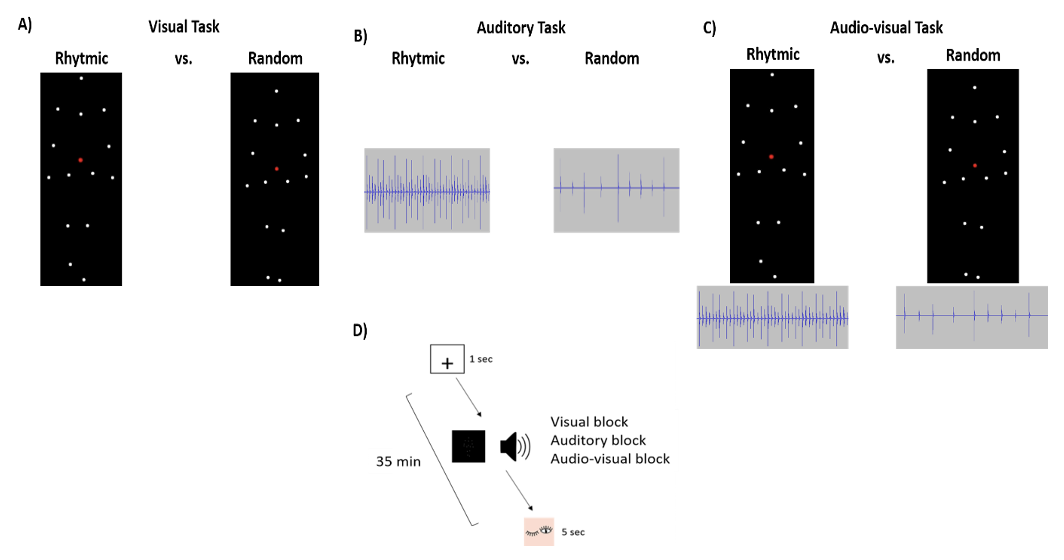
\includegraphics[width=0.85\textwidth]{appendix/Picture 1.png}
        \caption{Auditory, visual, audiovisual inputs, and the experimental timeline}
        \label{fig: visual stimuli}
\end{figure} 
Moreover, after the observation of each sensory input, six subjective report questions were presented: they referred to how the participant felt while seeing the point-light figure walking or listening to the footsteps sound. The questions had to be answered on a Likert scale with values between 1 (strongly disagree) to 5 (strongly agree) (see the Experimental Design section for further details and (Table \ref{tab: Behavioral questions})). 
The experimental task was developed using with \href{https://pstnet.com/products/e-prime/}{E-prime} software, which allowed us to build an experiment with different stimuli presentations (e.g. adding images, questions and text).

To measure the level of physical activity of each participant, which would be later correlated to the EEG results, we used the \textit{Active-Q} questionnaire (it can be found in the Appendix A.(\ref{pdf: Active-Q questionnaire})), which was created precisely to assess the total physical activity and inactivity in adults, through a series of multiple choice questions (referred to a one-year time) on daily activity, mean of transportation used, leisure and sports activities; and the time a day spent for each of them \parencite{Bonn_2012}. 
The questionnaire was translated in Spanish from the original English version and transformed from a PDF file into an interactive digital version using the platform \href{https://www.qualtrics.com/uk/?rid=ip&prevsite=en&newsite=uk&geo=ES&geomatch=uk}{Qualtrics}. 

\section{Experimental design}
The current study is a mix models study design presenting both auditory (footstep sound) and visual (walking point-light figure) inputs at the frequency rate of 2 Hz in a rhythmic or random sequence, in three different blocks (auditory, visual and audiovisual). The blocks were presented in a randomized order to all the participants. 
At the beginning of the experimental session, we included a text with the instructions and right afterwards a white fixation cross preceding each sensory input presentation. 
In each experimental block the sensory inputs were presented four times in rhythmic sequences and four times in random sequences, each sensory input presentation lasted 60 seconds. The sensory inputs were presented in rhythmic and random sequences in a random order within each experimental block.  

During the presentation of each sensory input an attentional task was set. For the auditory inputs, the participants had to detect changes of the pitch (to a more acute or grave footstep sound) in the footstep sound stimuli. For the visual and audiovisual inputs, the participants had to focus their attention on the central dot of the point-light-figure which changed from red to white. The participants had to report to the experimenter the number of changes in both pitch footstep sound and the color of the central dot after each sensory input presentation.  
Moreover, after each sensory input presentation the participants had to answer six subjective report questions in a 5-points Likert scale (see Table \ref{tab: Behavioral questions}). Finally, after answering the subjective report questions, an eye-blink figure was presented during fifteen seconds indicating that they had time to blink if needed (see Figure \ref{fig: visual stimuli} for the experimental block design).  
A break of roughly five minutes was taken between all blocks to fix the conductivity of the electrodes with a gel \footnote{The gel employed in the EEG procedure is a mix of salts and water that allows the conductivity between the scalp and the electrodes.} and to let the participants rest. Altogether, the experiment and the set-up of the EEG cap on the participants had a duration of almost two hours.

For what concerns the Active-Q questionnaire, it was administrated via e-mail a few days before the experiment, together with some additional information about the study.

\section{Procedure}
Before the experiment began the participants had to sign the informative consent, and they would ask questions if needed. Afterwards a careful preparation was made, where we placed the EEG cap on their head\footnote{The EEG cap was previously prepared with all the 64 electrodes in their relative site.}, the external on the side of the right eye and under it, as well as on the mastoids. Then a gel was inserted in each electrode (both external and placed on the cap) in order to diminish the impedance and allow a good signal connectivity. 
Additionally, if the participants had any trouble completing the Active-Q questionnaire at home, they were helped to do so before the start of the experimental session. 

The participants sat on a chair in front of the computer screen where the stimuli were displayed and wore headphones to listen to the auditory stimuli. They were asked to avoid moving and blinking when the sensory stimuli were presented to avoid noise signal in the EEG recording. 
After reading the instruction on the screen, the participants had to pay attention to the stimulus that was being presented and count the number of changes in the color of the point-light figure's central dot or in the tone of the footstep sounds. At the end of each stimulus, they were asked to tell the experimenter how many changes they were able to observe or hear through a speaker\footnote{The speaker was used to communicate with the participants, which were in a different room from the experimenters. Furthermore, they could be seen through a webcam, and make signs if anything was needed.}. 

Afterwards, the subject questions were presented and had to be answered by the participants using numbers from 1 to 5 on the keyboard placed in front of them. When a question was answered the following one was automatically shown. When all the six questions were completed the eye-blinking image was presented, this was inserted for the participants to yawn, blink or stretch their face muscles if needed; furthermore they were expressively told that they could do so also during the answering of the questions, since the EEG recording during those time was of no interest for our analysis.  

After all the eight stimuli with their relative questions were shown, a block was completed and a small break took place, where the participants were offered something to drink or eat and the electrodes' impedance was checked. 
When all the blocks were completed, the participants could wash their head from the gel in a sink.

\subsection*{Subjective report assessment scale}
For the subjective report questions presented at the end of each experimental block we used six question related to the participant's perception of the sensory inputs, which can be found in Figure \ref{tab: Behavioral questions}. 
We inserted these questions to understand the feelings produced by the sensory inputs; in particular we aimed to see if the perception of involvement with the sensory input or the positive feelings recognized during the presentation of such stimuli, could influence the level of neural entrainment related to that particular sensory input. Further, we wanted to understand if the difference of sensorimotor synchronization previously observed between the presentation of the stimuli presented in a rhythmic or random sequence (Matamala-Gomez et al. in preparation) could also be confirmed by a subjective report on their perception. 
For these purposes, we decided to insert two questions on the involvement of our body with the sensory stimuli presented (Q1 \textit{«I felt involved with the marching movement of the white dot figure during the video observation (it was as if I was also moving)»} and Q4, measuring agency \textit{«During the observation of the video, I felt like I was inside the body of the white dots (as if my own body was performing the movement)»}); two questions on the positive feelings evoked by the stimuli (Q5 \textit{«During the observation of the video, I had a pleasant sensation”} and Q6 \textit{«During the observation of the video, I felt relaxed»}); one on the fluidity of the stimuli (Q3 \textit{«The movement of the white dot figure seemed fluid to me.»}); and one on the perception of the rhythm, which was considered the most significative one (Q2 \textit{«The rhythm of the steps of the white dot figure seemed to reproduce the rhythm of my real march»}). 
All the questions were adapted for each different sensory input, and can be found in Figure \ref{tab: Behavioral questions}. 
Their score had to be given on Likert Scale from 1 (strongly disagree) to 5 (strongly agree). The results obtained from the questions were collected into a \textit{.txt} file by E-prime and inserted in an Excel table through a Python script, so that later they could be easily used to make statistical analysis. 
\begin{table}[H]
    \centering
    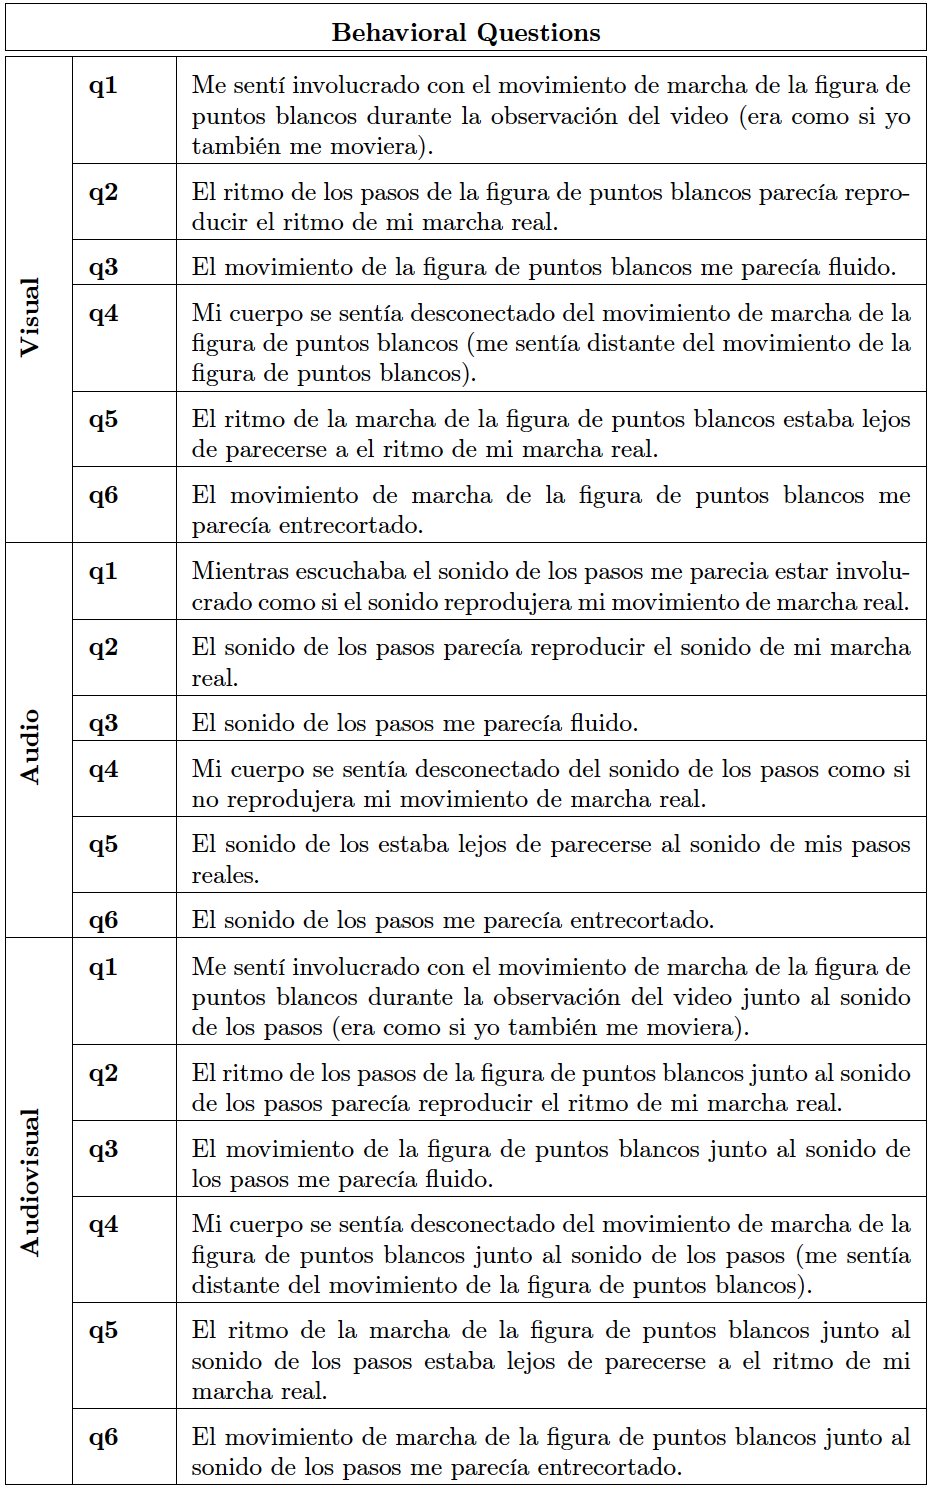
\includegraphics[width=0.65\textwidth]{appendix/questions.png}
    \caption{Table: Subjective report questions translated in English from Spanish}
    \label{tab: Behavioral questions}
\end{table}

Regarding the data for the Active-Q questionnaire (the questionnaire can be found in the Appendix \ref{pdf: Active-Q questionnaire}), we conducted the score calculation following the instruction reported on the article where it is explained, and its efficiency is tested \parencite{Bonn_2012}. Initially, we exported in an Excel file the results collected by Qualtrics with their numeric values (e.g. if the participant had selected the first option, the result would have been 1), this was imported in a Python file where the numeric values related to each activity were transformed into the MET values reported in Table A.\ref{tab: met_values}, which were encountered in the previously cited article. On the other hand, the frequency of each activity was measured multiplying the hours/minutes a day for the number of days per week; if a range of time was presented, we previously calculated the average of it, and then convert it into hours per day (e.g. the range 15-29 minutes/day was converted to 0.36 h/d).  
After creating an Excel table with the new scores accorded to MET values and the duration of hours/week, we proceeded to calculate the final Active-Q score, which returns a number of kilojoules per day, using the following formula: 
\[
\text{EE}_{\text{activity}} \, (\text{kJ/day}) = \text{MET}_{\text{activity}} \cdot \text{Weight} \, (\text{kg}) \cdot \text{Duration}_{\text{activity}} \, (\text{h/d}) \cdot 4.184
\]
The MET value and duration of the activity were multiplied by the weight of each participant (which was asked individually to the participant before the experiment), and the number 4.184, which is a conversion factor used to transform values from kcal to kJ. The obtained results represented the daily physical activity of each participant.

\section{Analysis}
\subsection{EEG data analysis}
The EEG data was registered through the software provided by \href{https://brainvision.com/applications/brain-vision-software/}{BrainVision} at the sampling rate of 1000 Hz; for all the subjects we made three different registrations, one per each experimental block (auditory, visual, and audiovisual). 
Before conducting the frequency-tagging analysis, the data was preprocessed using the \href{https://eeglab.org/}{EEGLAB toolbox} ran with Matlab: all the chunks of register that weren't necessary (i.e. the initial part with the instructions, the one related to the eye-blink figure and the ones corresponding to the subjective report questions) were trimmed. Later we re-referenced the data to channels 31 and 32, which correspond to the electrodes TP9 and TP10, positioned externally on the mastoids. Finally, we ran the Independent Component Analysis (ICA) to remove blinking and muscles artifacts and saved the preprocessed data into a new file. 

After the data for every block and for all the participants was preprocessed, we started the analysis with the help of some scripts made for the previous study and adjusted according to our necessities. 
Firstly, we extracted the epochs from the processed data: epochs of 20 seconds were obtained from the 60 seconds of each stimulus; the method of surface Laplacian and Current-Source Density (CSD) transform was applied to the data, dividing it between the one related to the rhythmic stimuli and to the random ones. 
From the files just generated, we computed spectral power activity with \href{https://www.fieldtriptoolbox.org/}{FieldTrip toolbox} of Matlab, using \textit{mtmfft} method, which allowed performing later analysis in time and frequency domains to study oscillatory brain activity and its modulation over time. The Fast Fourier transform (FFT) was applied to each sensory input (visual, audio and audiovisual) in both rhythmic and random sequences; therefore six variables were obtained. 

Using these variables we computed the averaged Signal-to-Noise Ratio (SNR), calculating the averaged signal-to-noise ratio (SNR) and the mean power spectrum and its variance through the different frequencies. We also plotted the activity power spectrum to see how the neural synchronization to rhythm would change through frequencies, and to observe whether the desired peak amplitude activity at 2 Hz was present. 
For the activity power spectrum analysis we decided to take into considerations the different regions of interest (ROIs) of our experiment, concerning the Occipital, Temporal and Sensorimotor areas, respectively enhanced by visual and audio sensory inputs as well as motor synchronization. For the analyses, the three different ROIs included the following electrodes: Temporal (right: FT9, FT7, T7, TP7; left: FT10, FT8, T8, TP8), Sensorimotor (right: F5, F3, F1, FC5, FC3, FC1, C5, C3, C1; left: F2, F4, F6, FC2, FC4, FC6, C2, C4, C6), and Occipital (PO3, POz, PO4, O1, Oz, O2). 

Furthermore, in order to neutralize the effects that the side of the injury in stroke patients might have on our results, we decided to invert the location of the electrodes for the patients who suffered the lesion in right hemisphere, which were the minority. Doing so the topographies that were generated should result not affected by the different injured side of the brain and the left hemisphere becomes the Affected Hemisphere in the stroke group and the Right hemisphere would be the Unaffected hemisphere. The interpretation of the corresponding figures in the results' section should be in consideration this aspect.  

Finally, we observed the distribution of the power spectrum activity for each sensory input, in both rhythmic and random sequences for each experimental block when presenting the sensory input at 2 Hz, in healthy individuals and patients with stroke. Moreover, we also could observe the power spectrum activity difference between rhythmic and random sequences (Figures \ref{fig: 3D topographies control group} and \ref{fig: 3D topographies stroke group}). 

\subsection{Subjective report questions analysis}
For the subjective report questions, we analyzed the mean difference between rhythmic and random sequences in each experimental block (auditory, visual, and audiovisual) for each subjective report question of the questionnaire. Further, we also calculated the mean difference between healthy subjects and patients with stroke in both rhythmic and random sequences in each experimental block for each subjective report question (Figure \ref{fig: bar_visual_pop}). In specific, we used the Wilcoxon Signed-Rank test for non-normally distributed data or the paired T-test for normal distributed data. We tested the distribution of the data with the Shapiro–Wilk test.
% We inserted all of our statistic results for each group and sensory input into different Excel tables in order to build with them separate bar plots (with their corresponding error bars) to show graphically the comparison between the rhythmic and random condition. 
% Finally, we decided to achieve an additional comparison between the rhythmic and random condition in the two distinct population groups, building a single bar plot with the mean results of all the questions in the diverse stimuli in the two groups. 

%% ---- questionnaire analysis part 
On the other side, with the scores of the physical activity, obtained with the Active-Q questionnaire, we aimed to explore the relationship with the subjective report questions and the brain power spectrum. To that aim we used Spearman’s correlation test for non-parametrical data. 
For the correlations, a numerical value for each participant and condition representing the mean power spectrum activity of each specific ROI (temporal, sensorimotor, and occipital) during each sensory input exposure (auditory, visual, and audiovisual) only at rhythmic sequences, was extracted, in both healthy and patients with stroke. 
In order to see whether there was a relationship between the power spectrum activity and behavioral responses, we selected the question Q2 (see Table \ref{tab: Behavioral questions}), that was the one more related to the rhythmic perception of the sensory input presentation. 